
\section{Theorie}
\label{sec:Theorie}
\subsection{Bedeutung des Zustandsdiagrammes}
Ein Stoff kann verschiedene Phasen annehmen. Der Begriff der "Phase" beschreibt
 einen räumlich begrenzten Bereich eines abgeschlossenen System, in dem sich ein Stoff
  in einem homogenem Zustand befindet. Wichtige Phasen sind die Aggregatzustände.
  Wechselt der Stoff nun den Aggregatzustand ist dieser Vorgang eine Phasenumwandlung.
  Die einzelnen Phasen und ihre Übergänge lassen sich mithilfe Zustandsdiagrammes
   wie in Abb. \ref{fig:diagram} darstellen. Ihn ihnen werden Druck und Temperatur
    des Systems, in welchem sich der Stoff befindet, gegeneinander aufgetragen.
  \begin{figure}
	\centering
	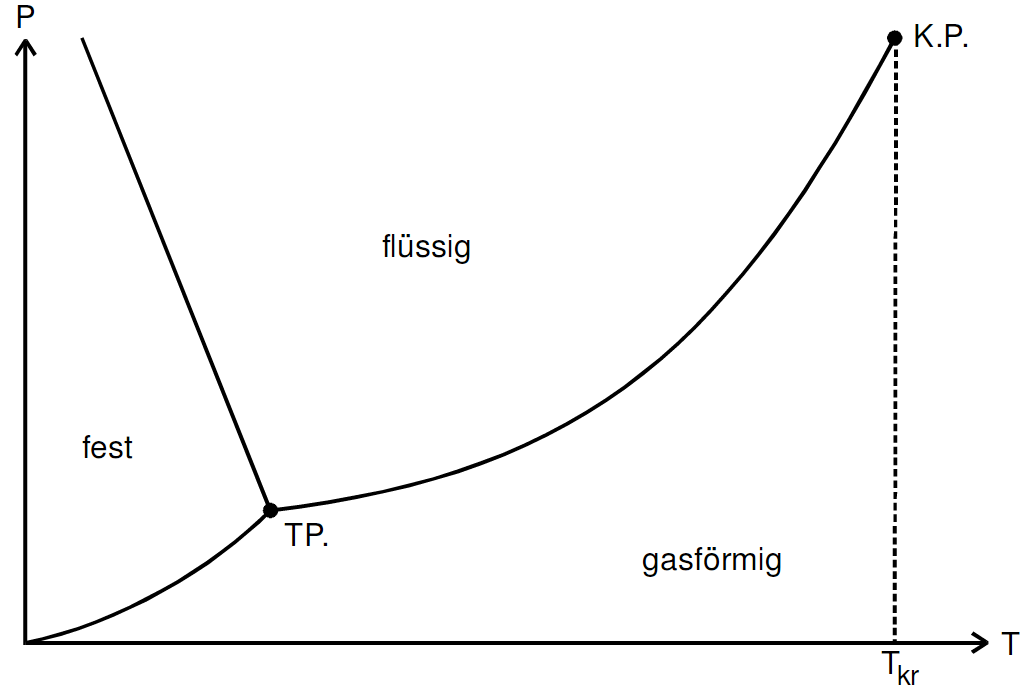
\includegraphics[width=\linewidth-150pt,height=\textheight-150pt,keepaspectratio]{content/Bilder/zustand.png}
	\caption{Eine qualitative Darstellung der einzelnen Aggregatzustände von Wasser\cite{V203}.}
	\label{fig:diagram}
\end{figure}
  Die Phase und das mögliche Verhalten des Stoffes hängen nun von den Parametern $P$ und $T$ ab.
  In den Flächen der Aggregatzustände können alle $P$ und $T$
   Kombinationen des jeweiligen Bereiches erreicht werden ohne das sich etwas an der Phase des Stoffes ändert.
    Liegen Die Koordinaten $(P,T)$ hingegen auf einer der Grenzlinien zwischen
    zwei Phasen, koexistieren Teilchen in beiden Zuständen.
    Dementsprechend hat das System auf diesen Linien nur noch einen Freiheitsgrad.
    Am Knotenpunkt aller Grenzlinien koexistieren zuletzt Teilchen aller Drei
     Zustände. Das System ist an diesem daher fest bestimmt.

     Im folgenden wird sich auf die Grenzkurve zwischen dem flüssigen und dem
      gasförmigen Zustand beschränkt. Diese heißt Dampfdruckkurve und wird hauptsächlich durch die
      Verdampfungwärme $L$ festgelegt.An ihrem oberen Ende liegt eine kritische
       Temperatur $T_\text{k}$ vor, bei welcher keine genaue Phase mehr angegeben werden kann. Es folgt ein näherer Blick auf die Vorgänge von
      Verdampfung und Kondensation im Vakuum.
\subsection{Vorgänge bei Verdampfung und Kondensation}
Wird eine Flüssigkeit in ein evakuiertes Gefäß gefüllt, so lässt sich eine
 Druckerhöhung im Bereich über der Flüssigkeit feststellen. Diese erfolgt, da ein Teil der
  Flüssigkeit in den gasförmigen Zustand wechselt. Die hierfür benötigte
   Energie $L$ muss entweder extern hinzugefügt werden oder sie wird der übrigen
    Flüssigkeit in Form eines Temperaturverlustes entnommen. Umgekehrt wird
     Energie bei Rückwechsel in den flüssigen Zustand wieder hinzugefügt. Es
      zeigt sich also ein Kreislauf. Nach hinreichend langer Zeit stellt sich
       ein Gleichgewicht zwischen Dampf und Flüssigkeit ein. Der dann vorherrschende
        Sättigungsdampfdruck hängt von der Temperatur ab und ist invariant
         unter einer Volumenänderung des Raumes. Bei letzterer
         verdampft oder kondensiert die nötige Flüssigkeitsmenge, sodass sich das Gleichgweicht wieder einstellt.
         \begin{figure}
         	\centering
         	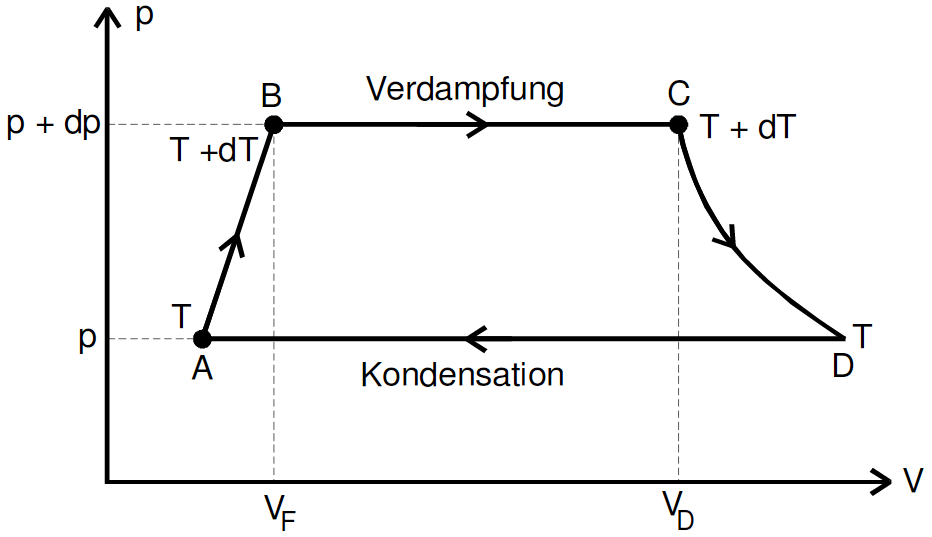
\includegraphics[width=\linewidth-150pt,height=\textheight-150pt,keepaspectratio]{content/Bilder/Kreislauf.png}
         	\caption{Eine mathematische Hilfsskizze zur Ermittlung der Funktion des Druckes auf der Verdampfungskurve\cite{V203}.}
         	\label{fig:Kreislauf}
         \end{figure}
         Stellt man den Kreisprozess nun mathematisch da, so wie in Abb. \ref{fig:Kreislauf} abgebildet, folgt die Clausius-Clapeyronsche Gleichung:
         \subsection{Lösung der Clausius-Clapeyronschen Gleichung}
         \begin{equation}
           (V_\text{D}-V_\text{F})\text{d}p = \frac{L}{T}\text{d}T \label{eq:DGL}
           \end{equation}
           mit dem Flüssigkeitsvolumen $V_\text{F}$ und dem Dampfvolumen $V_\text{D}$.
Diese lässt sich zunächst nur mit Schwierigkeiten lösen.
Liegen die verwendeten Temperaturen jedoch weit unterhalb von $T_\text{k}$ können
 einige Annahmen getroffen werden, die die Lösung vereinfachen.
\begin{itemize}
  \item $V_\text{F}$ ist zuvernachlässigbar klein gegenüber $V_\text{D}$.
  \item $V_\text{D}$ genügt der allgemeinen Gasgleichung $V_\text{D}(p,T) = R\frac{T}{p}$.
  \item Die molare Verdampfungswärme wird als konstant angenommen.
\end{itemize}
Mit diesen folgt für die Funktion des Druckes auf der Verdampfungskurve:
\begin{equation}
  p = p_0 \cdot exp \left(-\frac{L}{RT}\right) \label{eq:DGLLs}
\end{equation}
